% Theorie: Physikalische Grundlagen von Versuch/Messverfahren, Gleichungen ohne Herleitung knapp erklären
\section[Theorie]{Theorie \textnormal{\cite{scan}}}
\label{sec:theorie}

Das menschliche Gehör ist für Frequenzen von $\qty{16}{\hertz}$ bis $\qty{20}{\kilo\hertz}$ empfindlich. Unterhalb der Hörschwelle handelt es
sich um Infraschall, weit oberhalb liegen die Hyperschallfrequenzen. Von besonderem Interesse ist der Bereich von $\qty{20}{\kilo\hertz}$ bis
$\qty{1}{\giga\hertz}$. Dieser wird als Ultraschall bezeichnet und findet aufgrund seiner günstigen Eigenschaften zur zerstörungsfreien
Werkstoffprüfung sowie in der Medizin vielfältige technische Anwendungen.

\subsection{Grundlegendes Verhalten von Schallwellen}

Schall lässt sich grundsätzlich als longitudinale Druckwelle der Form
\begin{equation*}
	p(x,t) = p_0 + v_0 \hspace{0.2ex} Z \cos(\omega t - kx)
\end{equation*}
beschreiben, wobei $Z = c \hspace{0.2ex} \rho$ als akustische Impedanz oder auch Schallkennwiderstand bezeichnet wird.

\subsubsection{Geschwindigkeit}

Schallwellen teilen mit Phänomenen wie Reflexion und Brechung einige Eigenschaften der elektromagnetischen Wellen, die Phasengeschwindigkeit $c$
weist allerdings wegen Änderungen von Druck $p$ und Dichte $\rho$ im durchstrahlten Medium eine abweichende Materialabhängigkeit auf.
In Flüssigkeiten ist
\begin{equation*}
	c_l = \sqrt{\pfrac{1}{\raisebox{0.6ex}{$\kappa \rho \hspace{0.2ex}$}}}
\end{equation*}
mit der Kompressibilität $\kappa$ angegeben. Wegen auftretender Schubspannungen bilden sich innerhalb von Festkörpern auch Transversalwellen aus,
in diesem Fall bemisst
\begin{equation*}
	c_s = \sqrt{\pfrac{E}{\raisebox{0.6ex}{$\rho \hspace{0.2ex}$}}}
\end{equation*}
die Propagationsgeschwindigkeit des Schalls. Das Elastizitätsmodul $E$ nimmt hier die Rolle der reziproken Kompressibilität an, weshalb
die Schallgeschwindigkeit in Feststoffen im Allgemeinen richtungsabhängig ist.

\subsubsection{Übertragung}

Durch verlustbehaftete Interaktionen mit der Materie kommt es zur Absorption der Schallwelle, bei der die übertragene Energie in der Regel
exponentiell mit der Distanz $x$ über einen Term der Form
\begin{equation*}
	I(x) = I_0 \exp(\alpha x)
\end{equation*}
abfällt. Der Absorptionskoeffizient $\alpha$ verknüpft dabei die Ausgangsintensität $I_0$ mit der Intensität nach einer zurückgelegten Strecke.
An Grenzflächen wird ein Intensitätsanteil
\begin{equation}
	R = \left( \pfrac{Z_1 - Z_2}{Z_1 + Z_2} \right)^{\!\!\! 2}
	\label{eqn:reflexion}
\end{equation}
reflektiert, dieser Reflexionskoeffizient setzt sich aus den Impedanzen $Z$ der Grenzmedien zusammen. Die Transmission gehorcht
entsprechend $T = 1 - R$.

\subsection{Medizinische Anwendung von Ultraschall}

In der Medizin werden meist Kontaktmittel zwischen Schallgeber und Material verwendet, da Ultraschall stark von der Umgebungsluft
absorbiert wird. Auf diese Weise lassen sich dann Informationen über die innere Struktur durchstrahlter Materialien gewinnen. Die
beschriebenen Methoden lassen sich größtenteils auf die Werkstoffprüfung übertragen.

\subsubsection{Piezoelektrizität}

Wird ein elektrisches Wechselfeld parallel zu einer polaren Achse eines piezoelektrischen Kristalls geschaltet, kann dieser zu Schwingungen im
Ultraschallbereich angeregt werden. Abstimmung von Anregungs- und Eigenfrequenz erlaubt durch Resonanz das Erzeugen großer Wellenamplituden.
Verwenden dieses mit dem Begriff reziproker piezoelektrischer Effekt bezeichneten Phänomens ermöglicht die Nutzung extrem hoher
Schallenergiedichten. Über den umgekehrten Effekt dient der Piezokristall auch als Detektor, indem er durch eintreffende Schallwellen
in Schwingung versetzt wird. Wegen ihrer gleichbleibenden physikalischen Eigenschaften werden solche Messapparturen typischerweise
mithilfe von Quarzen realisiert.

\subsubsection{Scanverfahren}

Zur medizinischen Untersuchung von Körpern mittels Durchstrahlung werden häufig Laufzeitmessungen durchgeführt und ausgewertet.
Die verwendete Ultraschalltechnik besteht prinzipiell daraus, einen kurz Schallimpuls auszusenden und nach definierter Strecke
zu empfangen. Detektieren von Zeitintervall und Amplitude gibt so Aufschluss über den inneren Aufbau des Stoffes.

\paragraph{Durchschallung}

Wie in Abbildung \ref{fig:verfahren} zu erkennen, werden zum Durchschallungs-Verfahren Schallsignale ausgesendet und auf der gegenüberliegenden
Seite der Probe empfangen. Falls dazwischen Fehlstellen liegen, kann deren Einfluss in Form einer abgeschwächten Intensität am Ultraschalldetektor
gemessen werden. Diese Methode lässt jedoch keine Rückschlüsse über Tiefe und Form der Störquelle zu.

\paragraph{Impuls-Echo}

Anhand Abbildung \ref{fig:verfahren} wird deutlich, dass zur Anwendung des Impuls-Echo-Verfahrens der Ultraschallsender auch als Empfänger fungiert.
Der ausgesendete Puls wird dazu nach \eqref{eqn:reflexion} an Fehlstellen reflektiert, das resultierende Echo lässt sich aufzeichnen und bewerten.
Dessen Höhe gibt Aufschluss über die räumliche Ausdehnung der Fehlstelle, bei bekannter Schallgeschwindigkeit folgt mit
\begin{equation}
	s = \pfrac{1}{2} \hspace{0.2ex} c \hspace{0.2ex} t
	\label{eqn:strecke}
\end{equation}
die Lage innerhalb der Probe. Bei der Auswertung kommen in der Medizin verschiedene Darstellungsarten der Laufzeitdiagramme zum Einsatz.

\begin{figure}[H]
	\centering
	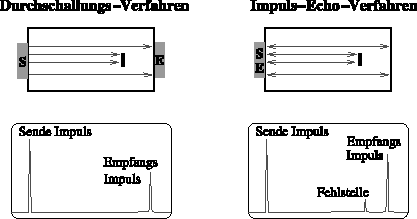
\includegraphics[width=0.6\linewidth]{content/grafik/verfahren.pdf}
	\caption{Exemplarische Signalverläufe und Impulsfolgen der Scanverfahren. \cite{scan}}
	\label{fig:verfahren}
\end{figure}

\paragraph{Darstellungsformen}

\begin{itemize}
	\item Der eindimensionale \textbf{Amplitude-Scan} (A-Scan) ermöglicht Strukturabtastung, indem die Amplitude des
	Echos gegen die Laufzeit aufgetragen wird.
	\item Zur Durchführung eines \textbf{Brightness-Scans} (B-Scan) wird die Ultraschallsonde über die Oberfläche der Probe bewegt, sodass sich
	ein zweidimensionales Schnittbild aufnehmen lässt. Dazu werden die Echoamplituden als Helligkeitsstufen angezeigt.
	\item Mit dem \textbf{Time-Motion-Scan} (TM-Scan) wird durch schnelles Abtasten zeitliche Auflösung gewonnen, um etwa die Bewegung
	eines Organs sichtbar zu machen. 
\end{itemize}


